%!TEX root = ../thesis.tex

% *****************************************************************************
% ********************************** CHAPTER 5 ********************************
% *****************************************************************************

\chapter[Implementation and Resulsts]{Implementation and Experimental Results}

In the concluding chapter of the thesis, the implementation details surrounding
important aspects of the system will be analyzed.
Also a comprehensive examination of the experimental results obtained from testing
the system in different situations will be performed.

\section{Message format}

In the context of embedded systems, the design choices for message
serialization and deserialization play a crucial role in the
overall efficiency and performance of the communication system.
The structure of the Message and the accompanying SerializeMessage and
DeserializeMessage methods demonstrate an attempt to balance the need for a
comprehensive representation of information with the constraints of the
underlying communication infrastructure.

The importance of having a low overhead in the message packets becomes
particularly evident when considering the limitations imposed by the RPMessage
library, which enforces a maximum message size of 1024 bytes.

\begin{figure}[H]
    \centering
    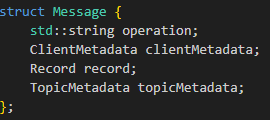
\includegraphics[width=0.5\textwidth]{Figures/implementation_message_format.png}
    \caption{Message Structure}
\end{figure}

The SerializeMessage function strives to achieve this optimization by
concatenating the essential fields of the Message structure into a single
string. This representation minimizes unnecessary padding or additional
metadata that might contribute to increased packet size.
Furthermore, the use of simple delimiters, such as commas, helps reduce the
overhead associated with encoding and decoding.

\begin{figure}[H]
    \centering
    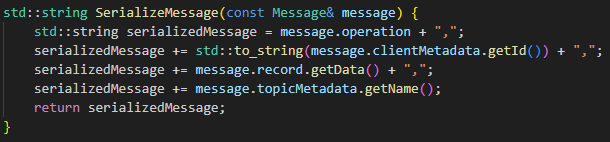
\includegraphics[width=1.0\textwidth]{Figures/implementation_serialize.png}
    \caption{Message Serialization}
\end{figure}

Additionally, the DeserializeMessage function efficiently extracts information
from the serialized string, ensuring that the deserialization process does not
introduce unnecessary complexities.

\begin{figure}[H]
    \centering
    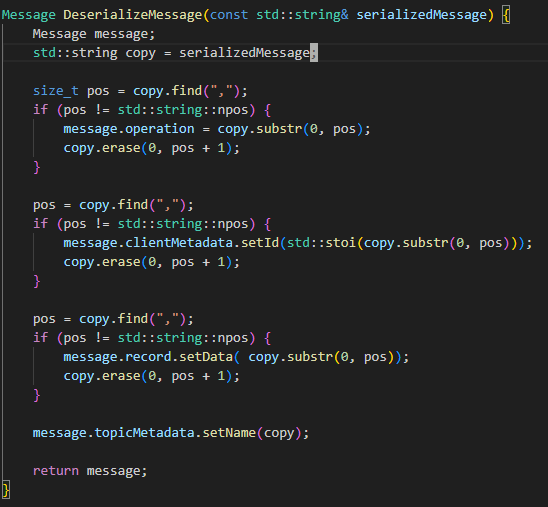
\includegraphics[width=0.7\textwidth]{Figures/implementation_deserialize.png}
    \caption{Message Deserialization}
\end{figure}

\section{Cluster information distribution}

The process of disseminating information about the position of brokers in the
system, as well as creating a vector containing details about topics, involves
the collaboration of two classes: SystemManager and TopicFactory.
This workflow is orchestrated to ensure that consumers and producers can access
relevant information about the cluster configuration efficiently.

The SystemManager follows these steps:

\begin{enumerate}
    \item   Initialization (SystemManager::init()): The SystemManager class is
        responsible for initiating the system. In this process, it starts by
        constructing a JSON request using the nlohmann/json library,
        specifying the operation as "getClusterInformation".
    \item Request to Configurer (CommunicationUtils::request): The constructed
        JSON request is then sent to a configurer, through a communication
        utility (CommunicationUtils::request).
    \item Parsing Response (json::parse): The response is then parsed using the
        nlohmann/json library, converting it into a JSON object. This object
        contains information about the cluster configuration, such as broker
        metadata and topic metadata.
\end{enumerate}

\begin{figure}[H]
    \centering
    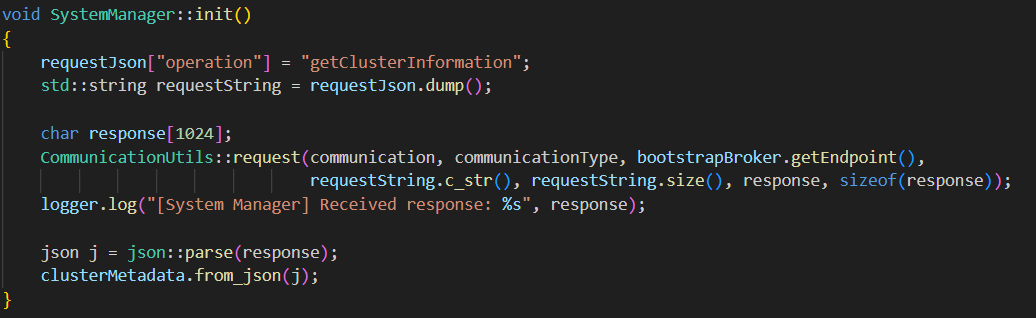
\includegraphics[width=1.0\textwidth]{Figures/implementation_system_manager.png}
    \caption{SystemManager requesting the state of the cluster to the configurer}
\end{figure}

The TopicFactoy is directly used by consumers and producers to retrieve the
information.

\begin{enumerate}
    \item   Creation of Topics (TopicFactory::createTopics()): The TopicFactory
        class utilizes the cluster information obtained by the SystemManager to
        create topics. It iterates through the broker metadata in the cluster,
        then for each broker, it iterates through the topics
        associated with that broker.
    \item   TopicProxy Instantiation: For each topic, a TopicProxy object is
        instantiated using the communicationType, BrokerMetadata,
        TopicMetadata, and a logger. The TopicProxy encapsulates functionality
        related to communication with the specified broker for the given topic.
\end{enumerate}

\begin{figure}[H]
    \centering
    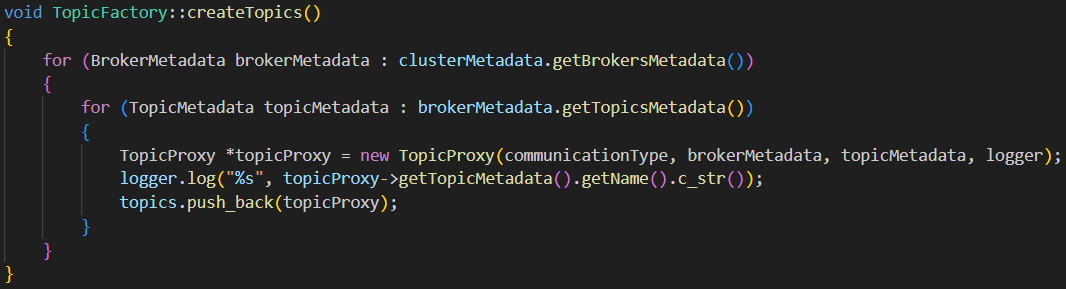
\includegraphics[width=1.0\textwidth]{Figures/implementation_topic_factory.png}
    \caption{TopicFactory creating a vector of Topics}
\end{figure}

\section{Broker mode}

In pub/sub systems, having both push and pull modes is essential
for serving different application scenarios. Push mode enables immediate
data dissemination to all subscribed consumers as soon as a record is received
by the broker, allowing for real-time updates and synchronous interactions.
On the other hand, pull mode allows consumers to retrieve data at their own
pace, providing them with the autonomy to fetch information when they are ready.

\begin{figure}[H]
    \centering
    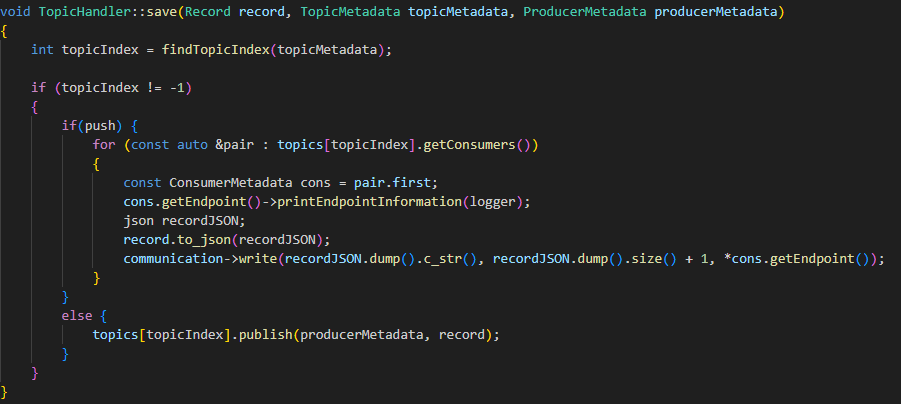
\includegraphics[width=1.0\textwidth]{Figures/implementation_broker_mode.png}
    \caption{Broker mode}
\end{figure}

The TopicHandler::save method plays a fundamental role in realizing this dual-mode
communication strategy. Upon receiving a record, the method dynamically adapts
its behavior based on the operational mode set for the broker.
In the push mode scenario, the method iterates through the consumers subscribed
to the relevant topic, sending the record individually to each consumer after
serialization.

In pull mode, the method delegates the received record to the publish method
of the corresponding topic.
This approach respects the asynchronous nature of pull-based communication,
allowing consumers to retrieve records at their convenience.

\section{Communiation}

In this section, the fundamental communication infrastructure will be explored.
RPMessageCommunication and RPMessageLinuxCommunication are the classes on which
most of the interactions are done in the system.
RPMessageCommunication specializes in real-time communication between cores,
ensuring low-latency data transfer.
Meanwhile, RPMessageLinuxCommunication extends this capability into the Linux
embedded environment, making sure communication remains robust through
RPMessage char devices.
Together, these components establish the basis for effective communication
across the different components.

\subsection{RPMessage}

The following implementation encapsulates the communication mechanisms using
RPMessage for real-time cores within the RPMessageCommunication class.
This class extends the more general Communication class and relies on the
RPMessage library to facilitate seamless interaction between cores. 

\begin{figure}[H]
    \centering
    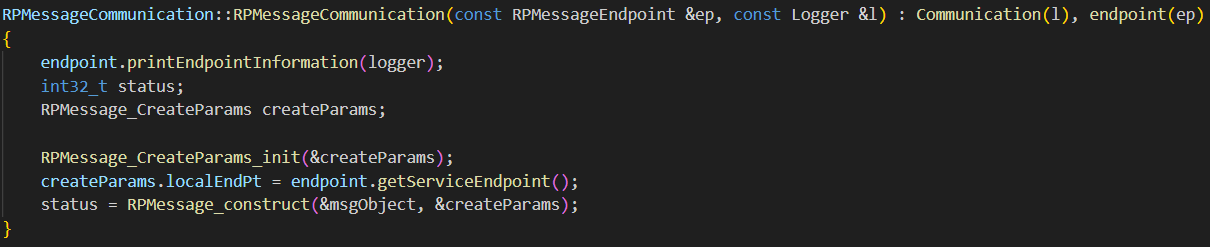
\includegraphics[width=1.0\textwidth]{Figures/implementation_rpmessage_init.png}
    \caption{Initialization of RPMessage}
\end{figure}

This constructor initializes a communication instance, setting the stage for
subsequent operations. It configures the RPMessageCommunication object with a
specific RPMessageEndpoint, creating a communication channel using the
RPMessage library.

\begin{figure}[H]
    \centering
    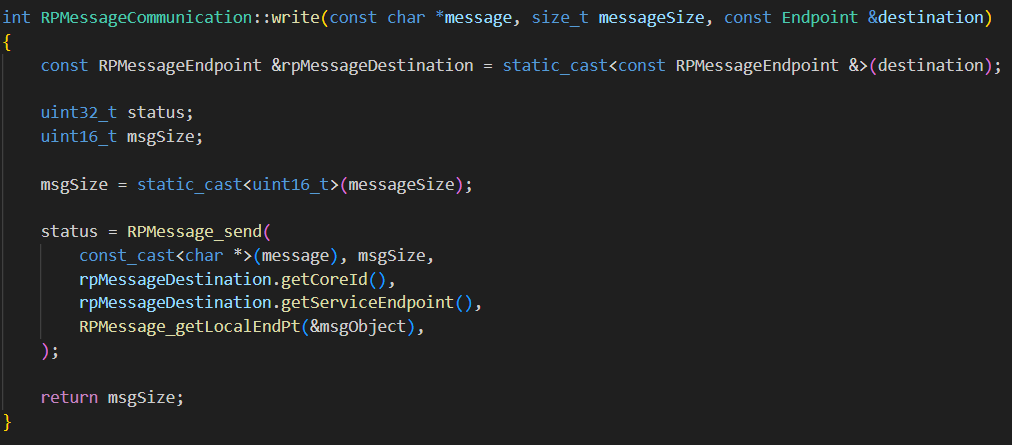
\includegraphics[width=1.0\textwidth]{Figures/implementation_rpmessage_write.png}
    \caption{Write method of RPMessage}
\end{figure}

Responsible for transmitting messages, the write method employs the RPMessage\_send
function to dispatch messages to a specified destination.
It extracts core ID and service endpoint details from the provided
RPMessageEndpoint. The return value signifies the size of the transmitted
message.

\begin{figure}[H]
    \centering
    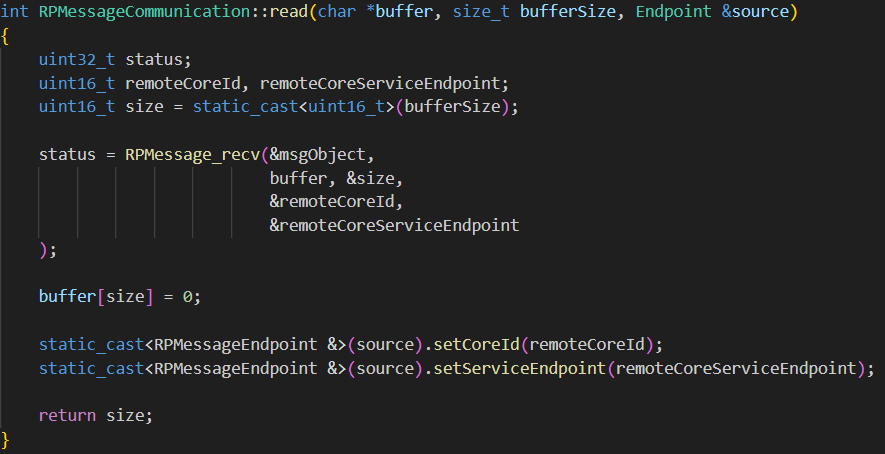
\includegraphics[width=1.0\textwidth]{Figures/implementation_rpmessage_read.png}
    \caption{Read method of RPMessage}
\end{figure}

Handling message reception, the read method utilizes the RPMessage\_recv
function to retrieve messages from the communication channel.
It extracts essential details such as the size of the received message,
the remote core ID, and the service endpoint.

\subsection{RPMessage for Linux embedded}

The write method within the RPMessageLinuxCommunication class facilitates the
transmission of messages from the current endpoint to a specified destination
in a Linux embedded environment using the RPMessage library.
Exploiting the RPMessage char device model, the method dynamically generates a
unique device name based on the destination's core ID and the current process
ID. It then checks if the destination is already present in the endpointMap.
If not, it opens a new RPMessage char device, updates the endpointMap,
and includes the associated file descriptor in the list of monitored file
descriptors. Subsequently, the method utilizes the send\_msg function to
transmit the message via the established communication channel, returning the
result of the transmission.
This implementation ensures efficient and reliable communication between
RPMessage endpoints in the Linux embedded system.

\begin{figure}[H]
    \centering
    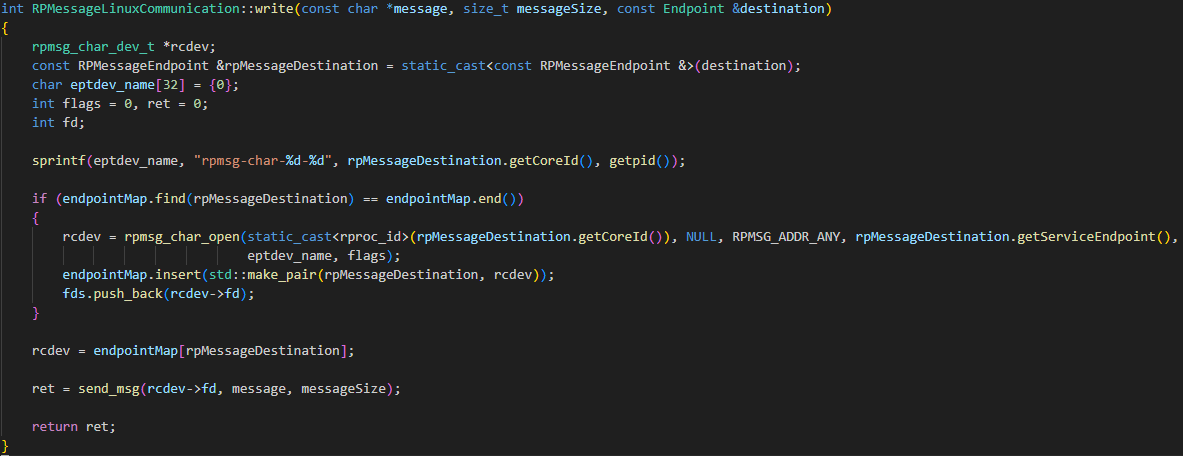
\includegraphics[width=1.0\textwidth]{Figures/implementation_rpmessage_linux_write.png}
    \caption{Write method of RPMessage for Linux embedded}
\end{figure}

The read method in the RPMessageLinuxCommunication class manages the reception
of messages in a Linux embedded environment using the RPMessage library.
Employing the select function, the method efficiently monitors a set of file
descriptors for incoming data. Upon detecting input availability, it identifies
the file descriptor with pending data, updates the source Endpoint accordingly
using the setSourceEndpoint function, and reads the message content via the
recv\_msg function.
This implementation ensures a responsive mechanism for message retrieval from
RPMessage endpoints within the Linux embedded system, balancing efficiency
and real-time considerations.

\begin{figure}[H]
    \centering
    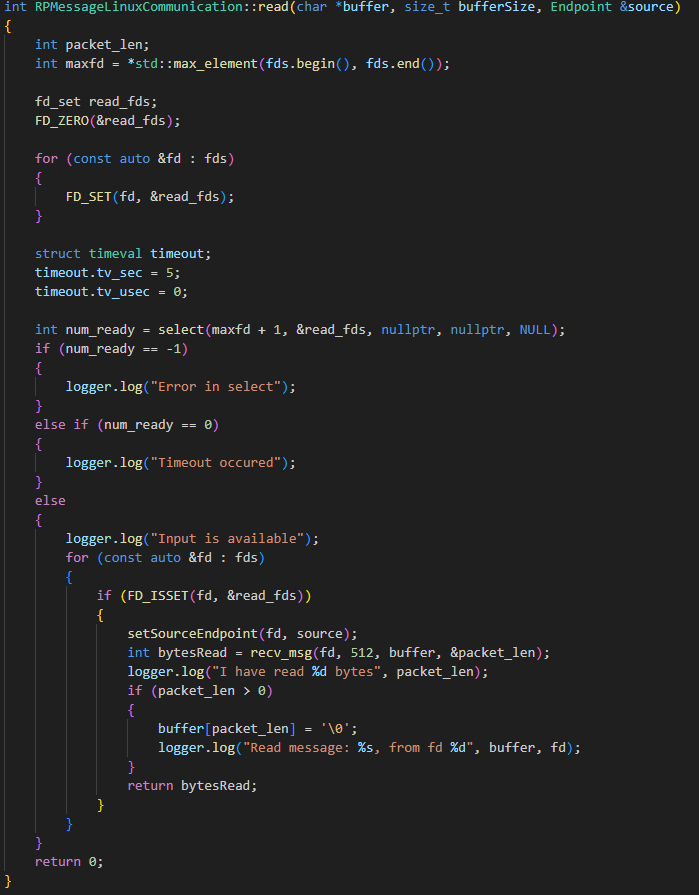
\includegraphics[width=0.8\textwidth]{Figures/implementation_rpmessage_linux_read.png}
    \caption{Read method of RPMessage for Linux embedded}
\end{figure}

\section{Results}

The last phase of the project involved the development and testing
the performance of the implemented system.
The focus of the testing was on measuring the time required for message
exchanges among different system elements.

Various tests were conducted, with the nature of each test contingent on the
processors involved in the communication.
The specific test performed include:

\begin{enumerate}
    \item   Time needed for the direct communication between real time cores
            and the Linux core.
    \item   Time needed for the exchange of messages using the implemented
            system varying in the processor used and in the number of
            consumers and producers.
\end{enumerate}

Throughout all tests, the size of the exchanged messages was varied to
understand the system performance under different conditions.

\subsection{Direct Communication}

The direct communication has been tested by using the Communication layer
realized previously.
Specifically, communication between different processors relied on the
RemoteProcessorMessage (RPMsg) function provided by Texas Instruments.
This API proves to be a robust solution for facilitating efficient
communication in a multi-core environemnt. RPMsg excels in establishing direct
communication channels between real-time cores and other cores within a
heterogeneous system. Leveraging this API ensures that the communication
channels are not only reliable but also characterized by low latency.

Within the RPMessage library, each packet is equipped with a 16 byte header,
shaping the structure of the communication. Consequently, the actual message
payload size is constrained by MAX\_MSG\_DIMENSION - 16 bytes.

\subsubsection{RTOS Cores}

Given the importance of real-time operations in embedded systems, the initial 
set of tests is about the direct communication of this kind of processors.
The processors which are taken into examination are the Cortex-R5F and the
Cortex-M4F.

The round trip time for R5s processors is computed by timing a message exchange
between two different R5s.
The round trip time for M4 processor is computed by timing a message exchange
between the M4 core and one of the R5s.

\begin{table}[H]
\centering
\caption{Round trip time results using RP Message between RTOS cores}
\label{table:direct_communication_RTOS_cores}
\begin{tabular}{lcccccc}
\toprule
Message Size (in bytes) & 32 & 64 & 128 & 256 & 512 & 1024 \\
\midrule
RTT R5 (in us) & 16.7 & 21.9 & 32.9 & 54.9 & 98.9 & 186.8 \\
RTT M4 (in us) & 35.7 & 48.2 & 73.2 & 125.7 & 228.1 & 435.7 \\
\bottomrule
\end{tabular}
\end{table}

With an increase in message dimension, a corresponding rise in Round Trip Time
(RTT) is anticipated, as indicated by the observed results. However, an
examination of table \ref{table:direct_communication_RTOS_cores} reveals a
non-linear relationship between message dimension and RTT.
The RTT demonstrates a slower growth rate as the message dimension increases.

\subsubsection{Linux and RTOS cores}

The results presented in Table \ref{table:direct_communication_linux_RTOS_cores}
are derived from message exchanges between real-time cores and the Cortex-A53
processor running Linux.
These tests hold particular significance as the more potent Cortex-A53 processor
serves as a centralized access point for various services.
It is imperative to ensure that the communication latency remains minimal.

In the Liux IPC library communication the maximum dimension for messages is
512 bytes.

\begin{table}[H]
\centering
\caption{Round trip time results using RP Message between Linux and RTOS cores}
\label{table:direct_communication_linux_RTOS_cores}
\begin{tabular}{lccccc}
\toprule
Message Size (in bytes) & 32 & 64 & 128 & 256 & 512 \\
\midrule
Linux and R5 (in us) & 50 & 61 & 77 & 108 & 168 \\
Linux and M4 (in us) & 64 & 80 & 110 & 177 & 306 \\
\bottomrule
\end{tabular}
\end{table}

\subsection{Broker Communication}

In this section there are the measurements obtained by using the pub/sub
middleware. There are two modes which are tested:

\begin{itemize}
    \item   Push: after that a producer sends a message to a broker, the broker
            sends it directly to all the subscribed consumers.
    \item   Pull: the consumers have to ask for the message to be delivered.
\end{itemize}

\subsubsection{RTOS cores}

Following the idea behind the tests done for the direct communication, also in
the broker communication the first processors which are tested are real-time
processors (Cortex-R5F and Cortex-M4F).

\subsubsection{Push}

When there is only one consumer and one producer in push mode the time needed
for the consumer and the producer are similar.
This result is expected given that the consumer is only expecting to receive
messages.

\begin{table}[H]
\centering
\caption{Round trip time results using the middleware between RTOS cores in
         push mode}
\label{table:broker_communication_RTOS_cores_push}
\begin{tabular}{lcccccc}
\toprule
Message Size (in bytes) & 32 & 64 & 128 & 256 & 512 & 1024 \\
\midrule
Producer R5 Time (in us) & 73.9 & 90.4 & 121.7 & 182.7 & 317.4 & 501.1 \\
Producer M4 Time (in us) & 99.7 & 111.1 & 137.6 & 190.7 & 322.4 & 506.9 \\
Consumer R5 Time (in us) & 76.9 & 92.9 & 122.9 & 182.9 & 317.6 & 503.2 \\
Consumer M4 Time (in us) & 74.9 & 92.1 & 120.6 & 182.8 & 315.2 & 570.3 \\
\bottomrule
\end{tabular}
\end{table}

As it can be seen in the table \ref{table:broker_communication_RTOS_cores_push},
the time for the consumer on the M4 is the same for the consumer on the R5 core,
since no messages have to be sent from the consumer when the communication is
in push mode.

\begin{table}[H]
\centering
\caption{Round trip time results using the middleware between RTOS cores with
         multiple consumers in push mode}
\label{table:broker_communication_RTOS_cores_multiple_consumers_push}
\begin{tabular}{lcccccc}
\toprule
Message Size (in bytes) & 32 & 64 & 128 & 256 & 512 & 1024 \\
\midrule
Producer Time (in us) & 277.2 & 300.9 & 358.9 & 478.2 & 744.9 & 1110.1 \\
Consumer 1 Time (in us) & 282.2 & 306.1 & 364.1 & 483.2 & 750.1 & 1115.1 \\
Consumer 2 Time (in us) & 763.4 & 765.4 & 804.1 & 991.4 & 1279.1 & 1503.4 \\
Consumer 3 Time (in us) & 539.4 & 510.1 & 634.6 & 754.2 & 1063.6 & 1283.4 \\
\bottomrule
\end{tabular}
\end{table}

The variations in time measurements among different consumers, which can be
seen in \ref{table:broker_communication_RTOS_cores_multiple_consumers_push}
can be attributed to the system's booting sequence.
During the boot process, the initialization of memory areas can differ,
consequently leading to variations in the prioritization of message delivery.
It becomes apparent that the order in which processes are booted significantly
influences the subsequent behavior of the system, resulting in different timing
outcomes across consumers.

\subsubsection{Pull}

Pull communication necessitates a higher volume of message exchanges as
consumers explicitly request records to be sent to them.
Despite this increased messaging overhead, pull communication offers several
notable advantages. Notably, it provides the flexibility for consumers to
process messages only when the core is ready, eliminating the need for message
buffering when the consumer is unable to process the message at a given time.
This on-demand processing capability enhances efficiency and resource
utilization. Additionally, pull communication simplifies the implementation
of Quality of Service (QoS) features, allowing for more precise control and
customization of message delivery based on the dynamic requirements of the
system. These advantages collectively contribute to the appeal and practicality
of pull communication in scenarios where fine-grained control over data
retrieval and processing is important. 

\begin{table}[H]
\centering
\caption{Round trip time results using the middleware between RTOS cores in
         pull mode}
\label{table:broker_communication_RTOS_cores}
\begin{tabular}{lcccccc}
\toprule
Message Size (in bytes) & 32 & 64 & 128 & 256 & 512 & 1024 \\
\midrule
Producer R5 Time (in us) & 93.1 & 104.1 & 121.2 & 152.4 & 212.7 & 301.8 \\
Producer M4 Time (in us) & 171.1 & 182.4 & 191.5 & 262.4 & 391.9 & 579.2 \\
Consumer R5 Time (in us) & 228.6 & 238.9 & 276.1 & 325.4 & 439.9 & 618.9 \\
Consumer M4 Time (in us) & 372.3 & 411.5 & 490.4 & 589.9 & 843.8 & 1236.7 \\
\bottomrule
\end{tabular}
\end{table}

\subsection{Linux on Cortex-A53}

Finally, the RTT for messages using the middleware in an heterogeneous
environment is tested, adding the Cortex-A53 with Linux to the real-time cores.

\subsubsection{Push}

\begin{table}[H]
\centering
\caption{Round trip time results using the middleware between Linux and RTOS
    cores in push mode}
\label{table:broker_communication_linux_RTOS_cores_push}
\begin{tabular}{lccccc}
\toprule
Message Size (in bytes) & 32 & 64 & 128 & 256 & 512 \\
\midrule
Producer Time(in us) & 98 & 127 & 191 & 264 & 393 \\
Consumer Time (in us) & 97 & 127 & 191 & 264 & 393 \\
\bottomrule
\end{tabular}
\end{table}

\subsubsection{Pull}

\begin{table}[H]
\centering
\caption{Round trip time results using the middleware between Linux and RTOS
    cores in pull mode}
\label{table:broker_communication_linux_RTOS_cores_pull}
\begin{tabular}{lccccc}
\toprule
Message Size (in bytes) & 32 & 64 & 128 & 256 & 512 \\
\midrule
Producer Time(in us) & 148 & 171 & 227 & 231 & 367 \\
Consumer Time (in us) & 264 & 292 & 322 & 406 & 565 \\
\bottomrule
\end{tabular}
\end{table}

\section{Result Analysis and future extensions}

The observed results in the experimental phase of the thesis reveal distinct patterns in the performance of the implemented pub/sub platform for embedded systems.

In the context of direct communication, the lower round-trip times (RTT) between real-time cores compared to those involving Linux cores underscore the efficiency of direct communication channels, particularly leveraging the RemoteProcessorMessage (RPMsg) framework. However, the middleware introduces additional services, contributing to a higher RTT. The intricacies of the Linux operating system and its IPC library, while providing a centralized access point for services, result in comparatively higher communication latencies.

Notably, the push mode in broker communication demonstrates symmetrical RTT for single consumers and producers, as expected, while variations in multiple consumer scenarios highlight the system's booting sequence impact. In pull mode, the flexibility and on-demand processing capability contribute to advantages despite increased messaging overhead. Overall, the results reflect a trade-off between direct communication efficiency and the richer feature set provided by the middleware, while Linux's higher RTT emphasizes the complexities introduced by the operating system.

For the end of the thesis, it is important to outline potential directions for
future investigations 

First and foremost, exploring the seamless integration of the pub/sub middleware with emerging edge computing paradigms represents a crucial direction. Investigating how the middleware can enhance communication efficiency and resource utilization in edge computing scenarios holds the potential to address the unique challenges presented by distributed computing at the network's periphery. 

Additionally, security and reliability enhancements are essential, with a focus on lightweight cryptographic protocols and fault-tolerant mechanisms to fortify communication channels and ensure system robustness.

Furthermore, the integration of artificial intelligence techniques with the pub/sub middleware offers an exciting frontier. Enabling intelligent data filtering, prediction, and adaptation in response to dynamic changes in the embedded environment can significantly elevate the platform's adaptability and responsiveness. 

Finally, the introduction of new protocols, potentially at an industrial level, can have a big impact in the automation industry. Such protocols can be customized to meet specific industry requirements, ensuring compatibility with diverse embedded applications and expanding the platform's utility in various domains.

